\chapter{Conversione del modello}

\section{Spiegazione rapida del modello originale}

Il modello esposto nel paper di riferimento è in realtà la combinazione di due CNN. Queste due reti vengono denominate
``Flow computation'' e ``Flow interpolation''. Entrambe le reti sono basate su un'architettura detta \emph{U-Net}, che
descrive una CNN formata da un encoder ed un decoder, entrambi composti da una gerarchia di diversi layer convoluzionali
e di pooling.
Entrambe le U-Net utilizzate hanno un encoder di 6 layer ed un decoder di 5 layer.

\begin{figure}[h!]
    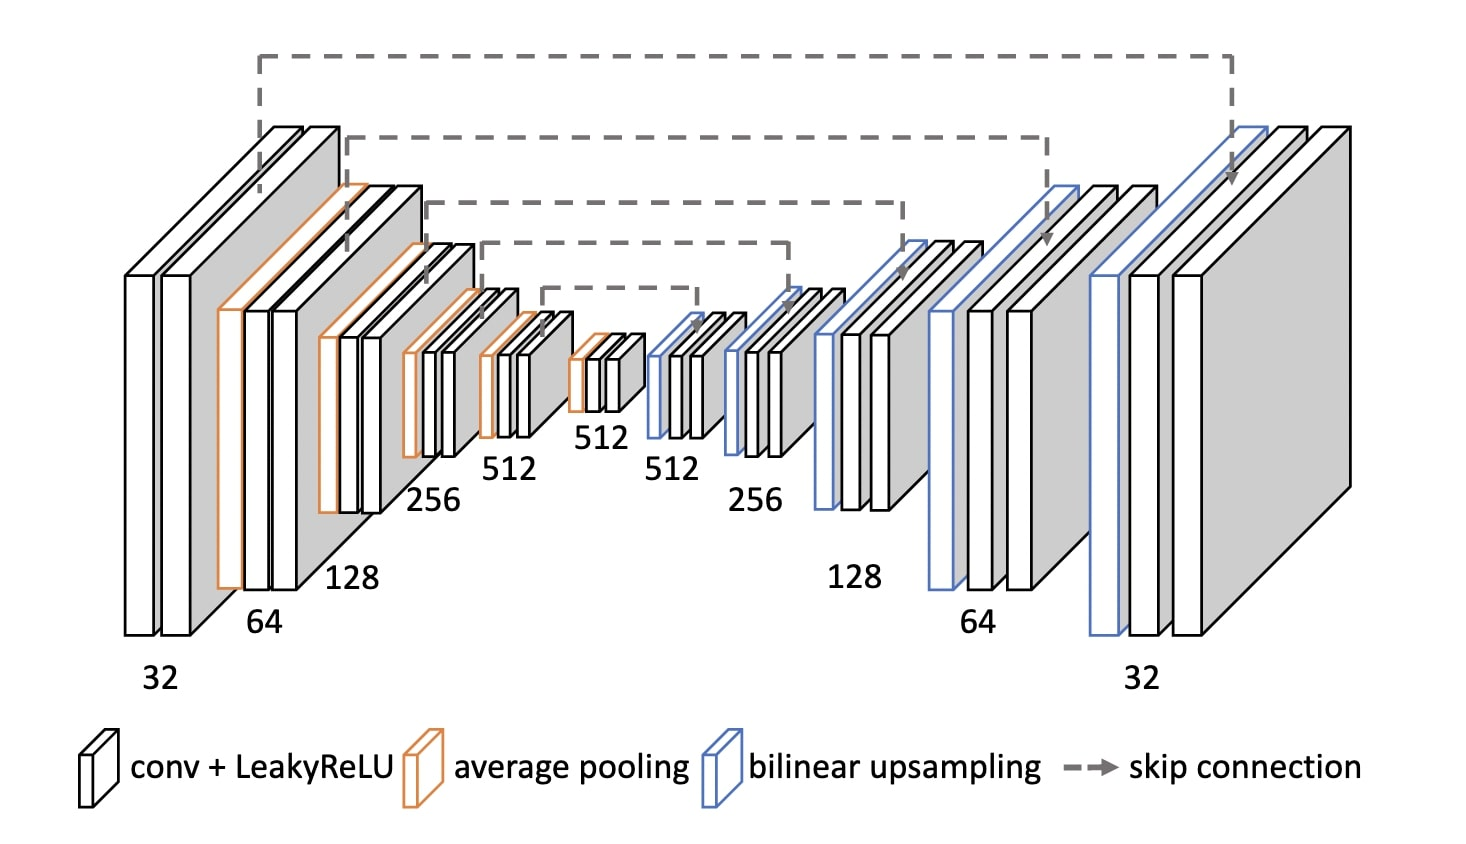
\includegraphics[width=0.7\textwidth]{img/architettura_slomo.jpg}
    \centering
    \caption{Illustrazione dell'architettura delle CNN Flow computation e Flow interpolation. Fonte: \cite{paper_superslomo}}
    \label{fig:architettura_slomo}
\end{figure}

Date due immagini $I_0$ e $I_1$ in input, l'obiettivo della rete è di stimare quale dovrebbe essere il flusso ottico tra 
il frame intermedio $I_t$ (non ancora generato) e le due immagini $I_0$ e $I_1$. Una volta completata la stima,
l'interpolazione (quindi la sintesi del nuovo frame) viene effettuata sulla base del flusso ottico mediante metodi 
algebrici descritti nel paper.

Il funzionamento della rete nel dettaglio non viene qui riportato, poiché risulta molto complesso e va oltre gli scopi
del seguente progetto.

\section{PyTorch e PyTorch Mobile}

PyTorch è uno dei due framework di machine learning più popolari.
Esso è sviluppato da Facebook (ora Meta), ed è basato su Python.

Il workflow del framework si può riassumere in questo modo:

\begin{itemize}
    \item Caricare i dati di training e test, come \texttt{Dataset}, 
    incapsulati poi dentro ad un \texttt{Dataloader} per permettere l'iterazione.
    \item Creazione di un modello, definendo i vari layer della rete neurale usando
    delle funzioni incorporate nel framework, dentro ad una classe \texttt{nn.Module}.
    \item Training, ripetendo delle iterazioni sul dataloader nelle quali si computa
    l'errore di predizione, e in base a esso si calcolano i nuovi pesi, per poi verificare
    il miglioramento dell'accuratezza tramite il dataset di test.
    \item Uso dei modelli così addestrati caricando i pesi e usando la stessa classe Module
    creata in precedenza, in modalità \emph{no\_grad} per differenziare dallo stato di
    training (impedendo così la modifica dei pesi), e ottenendo così delle predizioni.
\end{itemize}

PyTorch normalmente gestisce dati in forma di tensori, e offre funzioni di libreria per
convertire tipi di dato comune da e a tensori, in particolare, per lo scopo di questo
progetto, permette di convertire immagini in tensori e vice versa.

\subsection{PyTorch Mobile}

PyTorch Mobile\cite{sito_pytorch_mobile}\cite{doc_pytorch_mobile} è un runtime per PyTorch su dispositivi mobile e embedded, al momento in
beta. Supporta i sistemi operativi iOS, Android, e Linux, offrendo API per le operazioni
di uso comune necessarie a integrare le reti neurali in questo genere di applicazioni,
oltre a supportare operazioni di ottimizzazione come la quantizzazione. Offre anche 
un interprete ottimizzato per PyTorch su Android e iOS, che compila selettivamente solo
le componenti del framework necessarie all'app.

Si può anche sfruttare TorchScript per migliorare e facilitare l'ottimizzazione di modelli
a dispositivi mobile. TorchScript è un linguaggio creato ad hoc per PyTorch, ed è un sottoinsieme
del linguaggio Python, in particolare delle parti necessarie a rappresentare reti 
neurali. Inoltre, TorchScript ha tipi delle variabili statici, a differenza di Python.

PyTorch offre funzioni per compilare codice Python in TorchScript, sottostando a certi
vincoli. Per esempio, \texttt{torch.jit.script} permette di trasformare \texttt{Module}
o funzioni in \texttt{ScriptModule} e \texttt{ScriptFunction}, delle copie dell'originale
convertite in TorchScript, che poi potranno essere salvate tramite \texttt{torch.jit.save}
su file. In particolare, gli \texttt{ScriptModule} avranno gli stessi parametri del modello
originale, che verranno salvati su file insieme al modello, permettendo quindi di caricare
successivamente sia la logica che i parametri addestrati del modello dallo stesso file.

PyTorch Mobile sfrutta TorschScript per permettere di caricare il modello sul framework 
e nel linguaggio di destinazione (per esempio, Java o Kotlin per Android). Questo permette
di creare il modello usando l'API di PyTorch in Python, senza dover "ricreare" il codice
Python del modello originale in Java o altri linguaggi. Di conseguenza, l'API di PyTorch 
Mobile per Android è molto minimale, offrendo funzioni per caricare modelli di TorchScript, 
wrapper per tensori e modelli, e un wrapper generico ai tipi di TorschScript, \texttt{IValue}.

L'API non offre funzioni equivalenti alla maggior parte dei metodi di libreria PyTorch, 
supponendo che l'utente usi direttamente le funzioni in Python e le carichi nell'applicazione
convertite in formato TorschScript; l'API Mobile è quindi generalmente disaccoppiata dalla
libreria di Pytorch.

Il workflow generale per convertire modelli a PyTorch Mobile è descritto nella figura 
\ref{fig:workflow_pytorch_mobile}. Una volta ottenuto il modello convertito, e trasformati
i dati in \texttt{IValue} tensori nell'API del sistema di destinazione, si chiama il metodo
\texttt{forward} del modello convertito per ottenere la propria predizione.

Una nota importante è il diverso formato dei modelli TorchScript ottimizzati per mobile: 
essi vengono salvati tramite la funzione interna alla classe \texttt{ScriptModule}
\emph{\_save\_for\_lite\_interpreter}, in un formato diverso rispetto a quelli salvati tramite
\texttt{torch.jit.script}, come si evince dall'estensione suggerita dalla documentazione .ptl
invece di .pt. Nella versione attuale di PyTorch Mobile, esistono due versioni diverse della
libreria (per Android, \emph{org.pytorch.pytorch\_android} e 
\emph{org.pytorch.pytorch\_android\_lite}): ogni versione è in grado di caricare solo i file
TorchScript salvati dalla funzione corrispondente, e non dall'altra; questo al momento offre
problemi per la conversione di funzioni convertite a \texttt{ScriptFunction}, che attualmente
non dispone di un metodo \emph{\_save\_for\_lite\_interpreter}, impedendo quindi di caricare 
funzioni convertite a TorchScript in un contesto \emph{lite}. Quindi, l'unico modo di usare
le varie funzioni di libreria di PyTorch all'interno di applicazioni mobile, nella versione 
attuale, è usarle all'interno di un \texttt{Module} di rete neurale.

\begin{figure}[!bh]
    \centering
    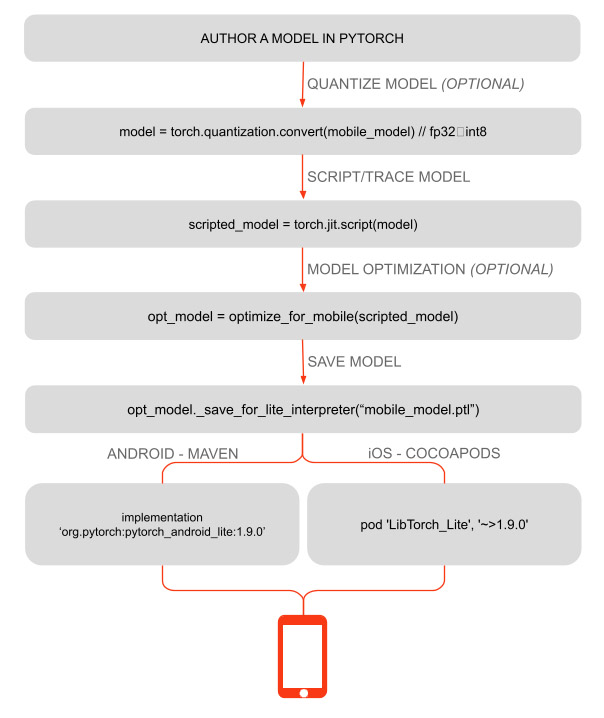
\includegraphics[width=0.7\textwidth]{img/pytorch_mobile_workflow.jpg}
    \caption{Fonte dell'immagine: https://pytorch.org/mobile/home/ \cite{sito_pytorch_mobile}}
    \label{fig:workflow_pytorch_mobile}
\end{figure}

\FloatBarrier

\subsection{Compensazione di lacune nell'API Mobile}

Come detto sopra, l'API di PyTorch Mobile, almeno su Android, è molto essenziale, assumendo
che l'utente farà il grosso della logica del modello in Python tramite PyTorch, per poi
convertirlo in TorchScript e caricarlo. Mancano quindi i vari metodi per manipolare tensori,
e gestire i set di dati, e nella versione attuale di PyTorch Mobile, come sopra, non è possibile
caricare funzioni TorschScript in un contesto di PyTorch Mobile lite. Nel caso in cui servano 
nell'applicazione funzionalità della libreria PyTorch all'esterno di un modello, sarà necessario
reimplementarle.

\subsubsection*{Dataset}
\label{sec:dataset}

In questo progetto è stato scelto di reimplementare la classe PyTorch \texttt{Dataset}, 
nel caso specifico di interesse al progetto, vale a dire un set di immagini rappresentanti
fotogrammi di un video, da caricare a due a due in ogni iterazione per interpolare i fotogrammi
tra esse. Questo permette di riprodurre il comportamento dell'implementazione originale di
SuperSlowMo in Python, usando un codice molto simile.

È stata quindi creata una classe \texttt{VideoDataset}, che implementa un'interfaccia 
\texttt{IDataset}, definite in maniera sintetica in seguito:

\begin{lstlisting}
public interface IDataset<T> extends Iterable<T> {
    public abstract T get(int index);
    public abstract int len();
}

public class VideoDataset<T> implements Dataset<Pair<T, T>> {
    private IImageLoader imageLoader;
    private String root;
    private String[] framePaths;
    private Function<Bitmap, T> transform;
    private Size origDim;
    private Size dim;

    public static <T> VideoDataset<T> withRootPath(String root, 
        Function<Bitmap, T> transform) {...}
    public static <T> VideoDataset<T> withContextAssets(Context context, 
        String root, Function<Bitmap, T> transform) {...}

    [...]
}
\end{lstlisting}

VideoDataset viene creata a partire da set di immagini (specificati o fornendo una cartella
nel file system Android, oppure una cartella negli asset dell'applicazione), e permette di 
fornire una funzione Transform che funziona in modo analogo all'argomento \emph{transform}
della classe \texttt{Dataset} di PyTorch: se presente, viene applicata su ogni immagine
durante l'iterazione del dataset, trasformandola in un tipo di dato diverso prima 
dell'elaborazione. 

Un uso comune di questa funzionalità è convertire immagini (classe
\texttt{Bitmap} in Android) in tensori, quindi \texttt{IValue} di tipo Tensore nell'API
PyTorch Mobile; l'API offre una funzione per questa conversione, 
\texttt{TensorImageUtils.bitmapToFloat32Tensor}. Un esempio di uso con \texttt{VideoDataset} 
è il seguente:

\begin{lstlisting}
videoFrames = VideoDataset.withRootPath(
    framesDir, 
    bitmap -> TensorImageUtils.bitmapToFloat32Tensor(bitmap,
        TensorImageUtils.TORCHVISION_NORM_MEAN_RGB,
        TensorImageUtils.TORCHVISION_NORM_STD_RGB
    )
);
\end{lstlisting}

Un ultimo punto importante riguardo a questa classe: in PyTorch, \texttt{Dataset} per video
ridimensiona le immagini caricate in modo che abbiamo valori di dimensione multipli di 32: per
esempio, da (320, 180) a (320, 160). È stato riprodotto questo comportamento in VideoDataset, ed
è stato rilevante in fase di conversione del modello a mobile (vedi 
\ref{sec:adattamento-modello}).

\subsubsection*{Concatenazione di Tensori}

Mancando le funzioni di PyTorch per svolgere operazioni tra Tensori, in particolare
\texttt{torch.cat}, in una prima versione del progetto era stato necessario reimplementare
questa funzione in Java. Non viene riportato il codice data la lunghezza, dovendo gestire 
separatamente i diversi casi di tipi primitivi contenuti dentro al tensore a causa della rigida
gestione degli array da parte di Java.

Nelle versioni successive del progetto, è stato possibile spostare tutto il codice che
necessitava di operazioni su tensori dentro al modello convertito in TorschScript, evitando
la necessità di reimplementare questa funzione.

\subsubsection*{Conversione da Tensori a Bitmap}

Come sopra, PyTorch Mobile offre una funzione per convertire immagini, quindi la classe
\texttt{Bitmap} nell'API Android, vale a dire \texttt{TensorImageUtils.bitmapToFloat32Tensor},
e alcune funzioni analoghe per altri tipi di dato del tensore. Notevolmente, nella versione 
attuale al momento dello sviluppo di questo progetto manca una funzione per la conversione
nella direzione opposta, vale a dire da tensore a immagine, cosa necessaria per reti neurali
che producono immagini come output, come questa.

È stato quindi necessario riprodurre questa funzionalità:

\begin{lstlisting}
public static Bitmap bitmapFromRGBImageAsFloatArray(float[] data, 
    int width, int height) {...}
\end{lstlisting}

Una prima versione portava a gravi artefatti nella conversione dello spazio RGB, che 
distorcevano le aree più luminose dell'immagine; la seconda versione, quella attuale, 
tiene conto della media e della deviazione standard dello spazio RGB di interesse in fase di
conversione, usando i valori forniti dall'API PyTorch Mobile, 
\texttt{TORCHVISION\_NORM\_MEAN\_RGB} e \texttt{TORCHVISION\_NORM\_STD\_RGB}. Un esempio di 
questo artefatto è in figura \ref{fig:img_conversion_error}.

\begin{figure}[!bh]
    \centering
    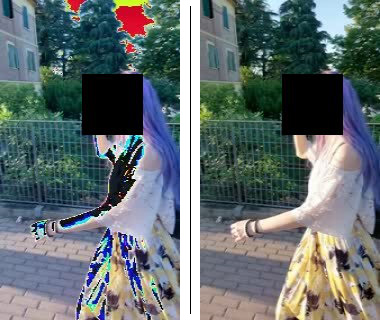
\includegraphics[width=0.85\textwidth]{img/conversione_img_errore.jpg}
    \caption{Errore nella conversione tensore $\rightarrow$ bitmap. A sinistra la prima versione, 
    a destra la versione corretta. Si noti la distorsione nelle aree luminose e le leggere
    differenze nella temperatura del colore.}
    \label{fig:img_conversion_error}
\end{figure}


\FloatBarrier

\section{Adattamento del modello a Pytorch Mobile}

Per adattare il modello di Super SlowMo a Pytorch Mobile innanzitutto è 
stato necessario convertire il codice di Python del modello originale in
Torchscript. Come spiegato nella sezione precedente, PyTorch Mobile è pensato
per scrivere la maggior parte della componente logica del modello direttamente in Python, 
per poi convertire la classe che estende \texttt{nn.Module} in Torchscript e esportarla nel
dispositivo mobile; questo soprattutto a causa dell'assenza di diverse delle funzioni necessarie
per il funzionamento del sistema dall'API Java.

\subsection{Struttura del sistema di partenza}

Le porzioni di codice seguenti estrometteranno le informazioni non essenziali.

\subsubsection*{Modello}

Il codice di Super SlowMo, seguendo il paper originale, usa tre diversi modelli PyTorch: 
\texttt{flowComp}, \texttt{ArbTimeFlowIntrp}, e \texttt{flowBackWarp}.

\begin{Python}
# Initialize model
flowComp = model.UNet(6, 4)
ArbTimeFlowIntrp = model.UNet(20, 5)
flowBackWarp = model.backWarp(videoFrames.dim[0], videoFrames.dim[1], device)
\end{Python}

Si noti come \texttt{flowBackWarp} viene creata con la stessa dimensione dei fotogrammi in 
ingresso. Queste sono istanze di classi \texttt{nn.Module} complesse così definite:

\begin{Python}
class UNet(nn.Module):
    """
    A class for creating UNet like architecture as specified by 
    the Super SloMo paper.
    """

    def __init__(self, inChannels, outChannels):
        [...]
        # Initialize neural network blocks.
        self.conv1 = nn.Conv2d(inChannels, 32, 7, stride=1, padding=3)
        self.conv2 = nn.Conv2d(32, 32, 7, stride=1, padding=3)
        self.down1 = down(32, 64, 5)
        self.down2 = down(64, 128, 3)
        self.down3 = down(128, 256, 3)
        self.down4 = down(256, 512, 3)
        self.down5 = down(512, 512, 3)
        self.up1   = up(512, 512)
        self.up2   = up(512, 256)
        self.up3   = up(256, 128)
        self.up4   = up(128, 64)
        self.up5   = up(64, 32)
        self.conv3 = nn.Conv2d(32, outChannels, 3, stride=1, padding=1)

    def forward(self, x):
        # Forward non riportato per ragioni di spazio, applica
        # i sotto-moduli creati sopra preceduti da due funzioni
        # ReLU e seguiti da una ulteriore funzione ReLU.

class backWarp(nn.Module):
    """
    A class for creating a backwarping object.

    This is used for backwarping to an image:

    Given optical flow from frame I0 to I1 --> F_0_1 
    and frame I1, it generates I0 <-- backwarp(F_0_1, I1).
    """

    def __init__(self, W, H, device):
        [...]
        # create a grid
        gridX, gridY = np.meshgrid(np.arange(W), np.arange(H))
        self.W = W
        self.H = H
        self.gridX = torch.tensor(gridX, requires_grad=False, device=device)
        self.gridY = torch.tensor(gridY, requires_grad=False, device=device)
        
    def forward(self, img, flow):
        # Extract horizontal and vertical flows.
        u = flow[:, 0, :, :]
        v = flow[:, 1, :, :]
        x = self.gridX.unsqueeze(0).expand_as(u).float() + u
        y = self.gridY.unsqueeze(0).expand_as(v).float() + v
        # range -1 to 1
        x = 2*(x/self.W - 0.5)
        y = 2*(y/self.H - 0.5)
        # stacking X and Y
        grid = torch.stack((x,y), dim=3)
        # Sample pixels using bilinear interpolation.
        imgOut = torch.nn.functional.grid_sample(img, grid)
        return imgOut
\end{Python}

\texttt{up} e \texttt{down} sono altri due moduli del sistema non riportati per ragioni di
spazio, riassunti dalla documentazione in questo modo:

\begin{verbatim}
down:
    A class for creating neural network blocks containing layers:
    Average Pooling --> Convolution + Leaky ReLU --> Convolution + Leaky ReLU
    This is used in the UNet Class to create a UNet like NN architecture.
up:
    A class for creating neural network blocks containing layers: 
    Bilinear interpolation --> Convolution + Leaky ReLU --> Convolution + Leaky ReLU
    This is used in the UNet Class to create a UNet like NN architecture.
\end{verbatim}

\subsubsection*{Interpolazione}

Il codice per l'interpolazione dei fotogrammi è contenuto nello script python 
\emph{video\_to\_slomo.py}.
Prima di tutto estrae i fotogrammi dal video tramite FFmpeg, un famoso programma per la 
conversione di file media. Carica poi i fotogrammi tramite un DataLoader:

\begin{Python}
# transform trasforma le immagini in tensori
videoFrames = dataloader.Video(root=extractionPath, transform=transform)
videoFramesloader = torch.utils.data.DataLoader(videoFrames, batch_size=args.batch_size, shuffle=False)
\end{Python}

Successivamente, itera sui fotogrammi presi a coppie tramite il \texttt{DataLoader}, interpolando i 
fotogrammi intermedi tramite i modelli creati in precedenza:

\begin{Python}
for _, (frame0, frame1) in enumerate(tqdm(videoFramesloader), 0):
    I0 = frame0.to(device)
    I1 = frame1.to(device)

    flowOut = flowComp(torch.cat((I0, I1), dim=1))
    F_0_1 = flowOut[:,:2,:,:]
    F_1_0 = flowOut[:,2:,:,:]

    # Save reference frames in output folder
    for batchIndex in range(args.batch_size):
        (TP(frame0[batchIndex].detach())).resize(videoFrames.origDim, Image.BILINEAR).save(os.path.join(outputPath, str(frameCounter + args.sf * batchIndex) + ".png"))
    frameCounter += 1

    # Generate intermediate frames
    for intermediateIndex in range(1, args.sf):
        t = float(intermediateIndex) / args.sf
        temp = -t * (1 - t)
        fCoeff = [temp, t * t, (1 - t) * (1 - t), temp]

        F_t_0 = fCoeff[0] * F_0_1 + fCoeff[1] * F_1_0
        F_t_1 = fCoeff[2] * F_0_1 + fCoeff[3] * F_1_0

        g_I0_F_t_0 = flowBackWarp(I0, F_t_0)
        g_I1_F_t_1 = flowBackWarp(I1, F_t_1)

        intrpOut = ArbTimeFlowIntrp(torch.cat((I0, I1, F_0_1, F_1_0, F_t_1, F_t_0, g_I1_F_t_1, g_I0_F_t_0), dim=1))

        F_t_0_f = intrpOut[:, :2, :, :] + F_t_0
        F_t_1_f = intrpOut[:, 2:4, :, :] + F_t_1
        V_t_0   = torch.sigmoid(intrpOut[:, 4:5, :, :])
        V_t_1   = 1 - V_t_0

        g_I0_F_t_0_f = flowBackWarp(I0, F_t_0_f)
        g_I1_F_t_1_f = flowBackWarp(I1, F_t_1_f)

        wCoeff = [1 - t, t]

        Ft_p = (wCoeff[0] * V_t_0 * g_I0_F_t_0_f + wCoeff[1] * V_t_1 * g_I1_F_t_1_f) / (wCoeff[0] * V_t_0 + wCoeff[1] * V_t_1)

        # Save intermediate frame
        for batchIndex in range(args.batch_size):
            (TP(Ft_p[batchIndex].cpu().detach())).resize(videoFrames.origDim, Image.BILINEAR).save(os.path.join(outputPath, str(frameCounter + args.sf * batchIndex) + ".png"))
        frameCounter += 1

    # Set counter accounting for batching of frames
    frameCounter += args.sf * (args.batch_size - 1)
\end{Python}

L'operazione è piuttosto complessa, e la quantità di fotogrammi generata dipende da 
\emph{args.sf}, lo \emph{scale factor}, vale a dire il moltiplicatore (intero) della quantità 
di fotogrammi del video finale a partire dall'originale. Per esempio, partendo da un video a 
30 fotogrammi per secondo, uno scale factor di 3 porterebbe a un video finale di 90 fotogrammi 
per secondo con la stessa durata, oppure ad un video finale di 30 fotogrammi per secondo ma 
lungo $\frac{1}{3}$ del video originale, in base al numero di fotogrammi per secondo desiderato.

\subsection{Adattamento}

Per adattare il complesso script di conversione e modello a PyTorch Mobile, è stato seguito il
workflow consigliato per questo runtime, facendo in modo di apporre meno modifiche possibili
al modello, per evitare possibili imprevisti sia data la sua complessità, sia dato lo stato 
ancora in sviluppo di PyTorch Mobile.

\subsubsection*{Adattamento del modello}
\label{sec:adattamento-modello}

Il modello è stato convertito in TorchScript e salvato su file per poterlo successivamente usare
nell'applicazione Android, come da workflow standard di PyTorch Mobile. Una prima versione
si limitava a creare istanze delle classi del sistema, convertirle in TorchScript dopo aver 
caricato i dati del modello pre-addestrato disponibile sul repository del sistema originale, 
e salvarle su file, in questo modo:

\begin{Python}
# ckpt: percorso file di checkpoint contenente 
# i parametri di training
dict1 = torch.load(ckpt, map_location='cpu')
flowComp = model.UNet(6, 4)
flowComp.load_state_dict(dict1['state_dictFC'])
flowComp_ts = torch.jit.script(flowComp)
flowComp_opt = optimize_for_mobile(flowComp_ts)
flowComp_opt._save_for_lite_interpreter('flowComp.ptl')
\end{Python}

Il procedimento ha funzionato, dopo delle minori correzioni necessarie data la staticità
dei tipi di TorschScript a differenza di Python, che portavano al fallimento della compilazione
a causa di linee di codice come

\begin{Python}
x = F.interpolate(x, scale_factor=2, mode='bilinear')
\end{Python}

dentro al modulo \texttt{up}, dove \emph{scale\_factor} richiede un dato di tipo \emph{float}, 
ma riceve un \emph{int}, cioè 2, come valore. Ovviamente questa linea è perfettamente valida in 
Python, che non differenzia neanche interi o float oltre a non avere questo genere di controlli
di tipo, ma non in TorschScript che appunto è un linguaggio a tipi statici.

Questa prima versione della conversione, però, per i problemi citati precedentemente nell'uso 
di funzioni di PyTorch al di fuori di un modulo rendeva difficile implementare la parte di 
valutazione che usava i modelli senza reimplementare diverse parti della libreria di PyTorch: 
quindi, si è optato per un approccio più vicino all'uso inteso del runtime Mobile, cioè di 
includere quanto possibile delle parti di codice riguardanti PyTorch all'interno dei moduli. 

Sono state quindi create due classi wrapper: \texttt{FlowCompCat}, che incapsula il codice
di valutazione eseguito prima di iterare su ogni fotogramma intermedio da interpolare, in
particolare la funzione \texttt{torch.cat} e lo \emph{splicing} dei tensori, che altrimenti
sarebbero dovuti essere reimplementati; e \texttt{FrameInterpolation}, che genera i fotogrammi 
intermedi (corrispondente al codice interno al loop \texttt{for intermediateIndex in 
range(1, args.sf)} nel codice di interpolazione originale).

\begin{Python}
class FlowCompCat(nn.Module):
    def __init__(self) -> None:
        self.flowComp = model.UNet(6, 4)

    def forward(self, t1, t2):
        flowOut = self.flowComp(torch.cat((t1, t2), dim=1))
        F_0_1 = flowOut[:,:2,:,:]
        F_1_0 = flowOut[:,2:,:,:]

        return (F_0_1, F_1_0)

    # Override di load_state_dict per caricare i dati del 
    # checkpoint dentro al modulo di flowComp interno, 
    # per cui sono stati creati
    def load_state_dict(self, state_dict: 'OrderedDict[str, Tensor]', strict: bool = True):
        return self.flowComp.load_state_dict(state_dict, strict)

class FrameInterpolation(nn.Module):
    def __init__(self, sizex, sizey) -> None:
        self.flowBackWarp = model.backWarp(sizex, sizey, 'cpu')
        self.ArbTimeFlowIntrp = model.UNet(20, 5)

    def forward(self, t: float, I0, I1, F_0_1, F_1_0):
        temp = -t * (1 - t)
        [...]
        # Codice corrispondente all'interno del loop nel codice 
        # di valutazione originale, fino all'assegnamento di Ft_p
        [...]

        return (wCoeff[0] * V_t_0 * g_I0_F_t_0_f + wCoeff[1] * V_t_1 * g_I1_F_t_1_f) / (wCoeff[0] * V_t_0 + wCoeff[1] * V_t_1)

    def load_state_dict(self, state_dict: 'OrderedDict[str, Tensor]', strict: bool = True):
        return self.ArbTimeFlowIntrp.load_state_dict(state_dict, strict)
\end{Python}

Questi moduli vengono poi convertiti a TorchScript, ottimizzati per l'interprete lite, 
e salvati su file come i precedenti.

Si noti come \texttt{FrameInterpolation}, che contiene al suo interno \texttt{flowBackWarp}, 
necessiti come esso di ricevere dall'esterno la dimensione dei fotogrammi. Questo ha creato una
ulteriore problematica nel convertire i modelli: infatti, mentre eseguendo lo script Python
l'oggetto del modulo \texttt{flowBackWarp} viene creato al momento, con parametri passati ad
hoc in base ai fotogrammi caricati durante l'esecuzione, i parametri del modulo da esportare
per PyTorch Mobile sono impostati prima della creazione del modulo da salvare, e una volta 
salvato su file rimangono costanti. Non è un problema per gli altri due moduli, che sono creati
con valori costanti per parametri. 

Per ovviare al problema, è stato necessario esportare un modulo diverso per ogni combinazione
di risoluzioni: questo mette già un primo vincolo all'applicazione mobile non presente
nel modello originale, vale a dire la possibilità di scegliere solo tra una limitata gamma di
risoluzioni di output.

Inoltre, dato il funzionamento dei \texttt{Dataset}, le immagini in elaborazione vengono 
ridimensionate a dimensioni multiple di 32 (vedi \ref{sec:dataset}); quindi le dimensioni 
preimpostate usate per la generazione dei moduli da caricare saranno assegnate a 
un valore compatibile con questo vincolo).

\begin{Python}
flowBackwarpResolutions = [
    (1280, 704),
    (320, 160),
]
flowBackWarps = {}

for res in flowBackwarpResolutions:
    key = f"frameInterp_{res[0]}x{res[1]}"
    flowBackWarps[key] = mobile_model.FrameInterpolation(res[0], res[1])
    flowBackWarps[key] = flowBackWarps[key].to(device)
    flowBackWarps[key].eval()
    flowBackWarps[key].load_state_dict(dict1['state_dictAT'])
\end{Python}

\subsection{Adattamento dell'interpolazione}

La valutazione, essendo eseguita dall'applicazione stessa, è realizzata in Java
tramite le API di Android e PyTorch. Viene usata la classe \texttt{VideoDataset} mostrata in
precedenza (vedi \ref{sec:dataset}) per emulare il caricamento dei fotogrammi dello script
originale:

\begin{lstlisting}
videoFrames = VideoDataset.withRootPath(extractedFramesDir.getAbsolutePath(), bitmap ->
    TensorImageUtils.bitmapToFloat32Tensor(bitmap,
        TensorImageUtils.TORCHVISION_NORM_MEAN_RGB,
        TensorImageUtils.TORCHVISION_NORM_STD_RGB
    )
);
\end{lstlisting}

È poi stata realizzata una classe \texttt{SlowMo}, contenente il \emph{core business} della
valutazione. Riceve dall'esterno il dataset, i moduli caricati da file, lo scale factor, 
un oggetto \texttt{ImageWriter} e parametri opzionali come un handler per gli aggiornamenti 
del progresso dell'operazione (per poterli mostrare sull'app) ed eventuali funzioni di log.

Anche \texttt{ImageWriter} è una classe dell'applicazione, usata per sostituire la creazione di
file di fotogrammi con eventuali funzioni mock, nel caso sia necessario in fase di test.

\begin{lstlisting}
slowMoEvaluator = new SlowMo()
    .scaleFactor(scaleFactor)
    .videoFrames(videoFrames)
    .flowCompCat(flowCompCat)
    .frameInterp(frameInterp)
    .imageWriter(new ImageWriter(convertedFramesDir.getAbsolutePath()));
\end{lstlisting}

Al suo interno, SlowMo ha una logica analoga a quella dello script \emph{video\_to\_slomo.py}
di partenza:

\begin{lstlisting}
int iter = 0;
int frameCounter = 1;
float progressIncrements = 1 / (float) videoFrames.len();
progress = 0;

for (Pair<Tensor, Tensor> sample : videoFrames) {
    IValue I0 = IValue.from(sample.first), I1 = IValue.from(sample.second);
    IValue[] flowOutTuple = flowCompCat.forward(I0, I1).toTuple();
    IValue I_F_0_1 = flowOutTuple[0], I_F_1_0 = flowOutTuple[1];

    // Save reference frames as image
    resizeAndSaveFrame(frameCounter, sample.first);
    frameCounter++;

    for (int intermediateIndex = 1; intermediateIndex < scaleFactor; intermediateIndex ++) {
        double t = intermediateIndex / (double) scaleFactor;
        IValue I_t = IValue.from(t);

        IValue I_Ft_p = frameInterp.forward(
                I_t,
                I0,
                I1,
                I_F_0_1,
                I_F_1_0
        );
        Tensor Ft_p = I_Ft_p.toTensor();

        // Save interpolated frame as image
        resizeAndSaveFrame( frameCounter, Ft_p);
        frameCounter++;
    }

    progress += Math.min(progressIncrements, 1f);
    publish(progress);
}
\end{lstlisting}

Quindi: per ogni coppia di fotogrammi, viene fatta un'elaborazione preliminare con
\texttt{flowCompCat}, e poi per ogni nuovo fotogramma la maggior parte del lavoro è svolto da
\texttt{frameInterp}, che crea il tensore corrispondente alla nuova immagine; esso viene a sua
volta convertito in Bitmap, scalato alla dimensione originale (per ovviare al già 
citato ridimensionamento in multipli di 32 compiuto da Dataset), e salvato come immagine.

\subsection{Limiti}

Il modello così adattato a mobile, per quanto ben più ottimizzato dell'originale grazie a
PyTorch Mobile e alle sue funzioni di ottimizzazione, rimane un software molto pesante per
dispositivi mobili. La versione attuale è stata testata su video a 180p (cioè, di dimensione
pari a 320x180 pixel, sia verticali che orizzontali), ma con dimensioni non troppo superiori
fallisce nell'esecuzione a causa della mancanza di memoria. Inoltre, i tempi di esecuzione
sono purtroppo lunghi, soprattutto aumentando la durata del video. Per il prototipo sviluppato 
nel corso di questo progetto, quindi, sono supportati video a 180p, con uno \emph{scale factor} 
di 2, che corrisponde a un raddoppiamento dei fotogrammi per secondo del video, o a un
rallentamento del 50\%.

Potrebbero essere svolte ulteriori ottimizzazioni, che saranno trattate successivamente 
in questa relazione (vedi \ref{sec:sviluppi-futuri}).
